\chapter{Тестирование ПО для суперкомпьютерного моделирования движения жидкости}

% \section{Анализ эффективности}

% Ускорение CPU

% Ускорение GPU/CPU

% \section{Сравнение солитонной волны с аналитическим решением}

% \section{Трёхмерная задача о разрушении дамбы}

%%%%%%%%%%%%%%%%%%%%%%%%%%%%%%%%%%%%%%%%%%%%%%%%%%%%%%%%%%%%%%%%%%%%%%%%%%%%%%%%%%%%%%%%%%%%%%%%%%%%%%
\section{Погрешности в дисперсионном соотношении}
%%%%%%%%%%%%%%%%%%%%%%%%%%%%%%%%%%%%%%%%%%%%%%%%%%%%%%%%%%%%%%%%%%%%%%%%%%%%%%%%%%%%%%%%%%%%%%%%%%%%%%

При моделировании гравитационных волн на поверхности воды, 
применяется поршень с уравнением движения второго порядка~\ref{eq:nwm_2nd}.
%
Входными параметрами модели являются длина волны $L$, высота волны $H$ и начальная фаза генератора $\phi_{0}$.
Глубина $d$ определяется поиском по частицам перед началом эксперимента.
%
Расчётный модуль определяет по данным параметрам волновое число (формула~\ref{eq:k_from_L}),
и далее, через дисперсионное соотношение (формула~\ref{eq:dis1}) определяет частоту.

\begin{equation}\label{eq:k_from_L}
    k = \frac{2 \pi}{L}.
\end{equation}

\begin{equation}\label{eq:dis1}
    \omega^{2} = gk \tanh(kd).
\end{equation}

Однако реальные частота и волновое число в численной модели может отличаться от аналитических значений.
%
Чтобы установить погрешности, проведена серия экспериментов с основными параметрами, представленными в таблице~\ref{t:params_dis}.

\begin{table} [htbp]
    \centering
    \begin{threeparttable}
        \caption{Основные экспериментов по моделированию гравитационных волн.}\label{t:params_dis}
        \begin{tabular}{| p{10cm} || c | c |}
            \hline
            Параметр   &  Обозначение  & Значение \\
            \hline
            \hline
            Количество частиц & $N$ & 700'000 \\
            \hline
            Длина сглаживания, м & $h$ & 0.02 \\
            \hline
            Глубина воды, м & $d$ & 1 \\
            \hline
            Высота волны, м & $H$ & 0.1 \\
            \hline
            Коэффициент искусственной вязкости & $\alpha$ & 0.01 \\
            \hline
            Коэффициент усреднения скорости & $\varepsilon$ & 0.001 \\
            \hline
            Искусственная скорость звука, м/с & $c_{0}$ & 62.6 \\
            \hline
        \end{tabular}
    \end{threeparttable}
\end{table}

На рисунке~\ref{f:dis_t_l3_x2} представена зависимость уровня жидкости в точке с координатой $x=2$ м. от времени.
%
Точками на рисунке обозначены результаты вычислений.
%
С помощью синусоидальной регрессии вычислены параметры установившихся волн, 
и восстановлена их функция (обозначена линией) следующего вида:
\begin{equation}
    \eta(t)=A \cos(\omega t + \phi_{0}) + d.
\end{equation}

\begin{figure}[h!]
    \centering
    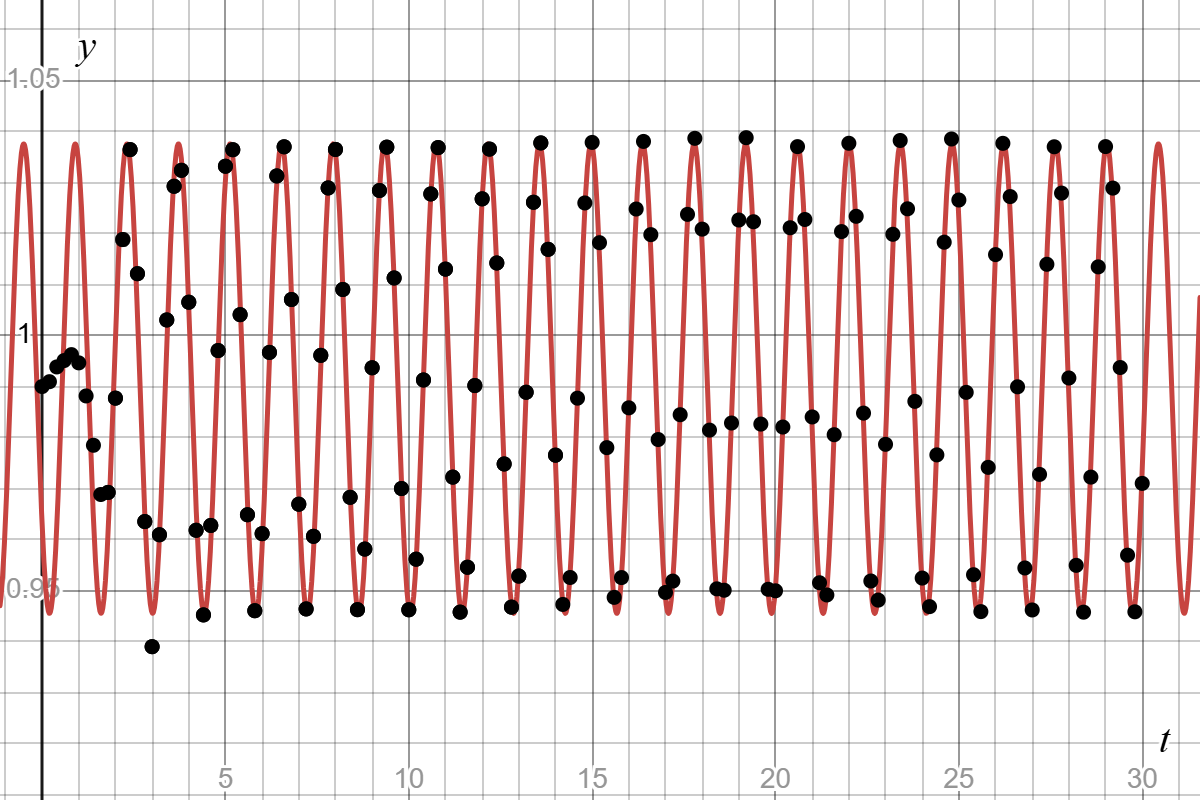
\includegraphics[width=0.7\textwidth]{images/dis_t_l3_x2.png}
    \caption{Зависимость уровня жидкости в точке с координатой $x=2$ м. от времени.}
    \label{f:dis_t_l3_x2}
\end{figure}

Одновременно проводится другой анализ --- строится зависимость уровня жидкости в определённый момент времени от координаты.
%
Пример такой зависимости представлен на рисунке~\ref{f:dis_x_l3_t30}. 
%
Для неё так же строится синусоидальная регрессия, и восстанавливается функция вида:
\begin{equation}
    \eta(x)=A \cos(kx + \phi_{1}) + d.
\end{equation}

\begin{figure}[h!]
    \centering
    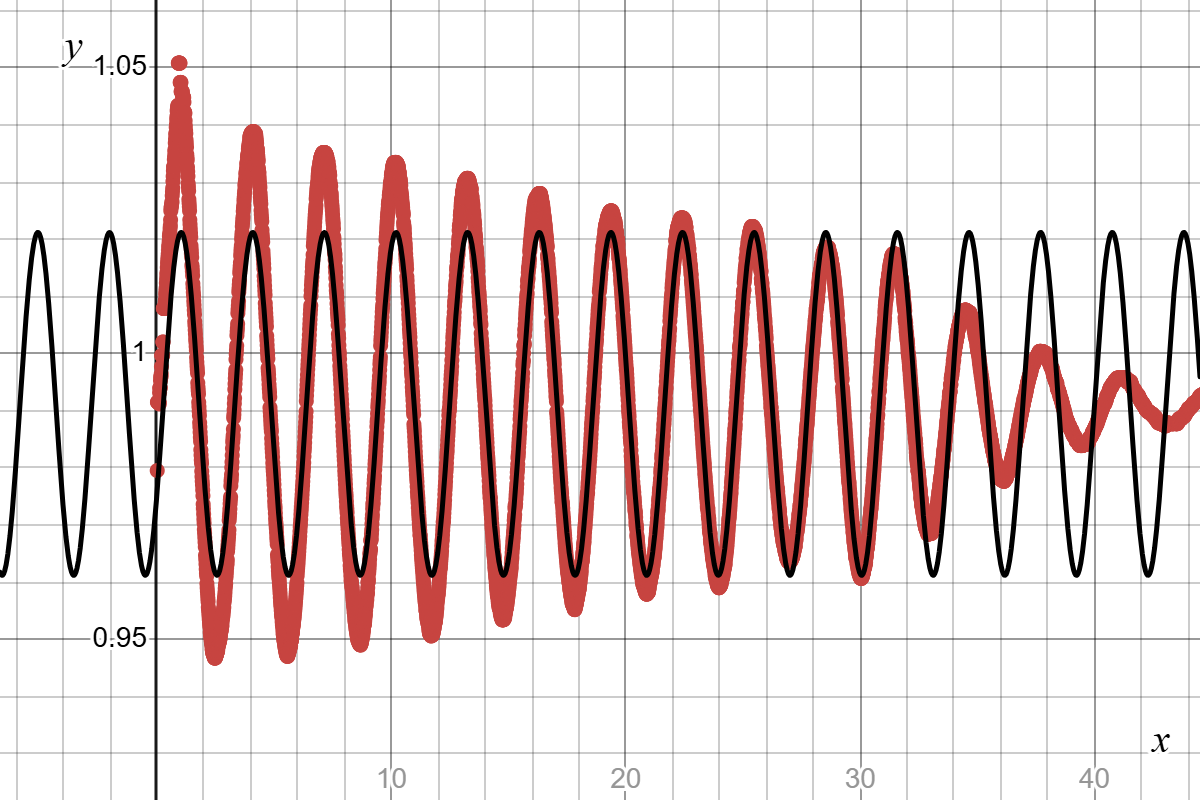
\includegraphics[width=0.7\textwidth]{images/dis_x_l3_t30.png}
    \caption{Зависимость уровня жидкости в момент времени $t=30$ с. от координаты.}
    \label{f:dis_x_l3_t30}
\end{figure}

На данных рисунках представлены расчёты для длины волны $L=3$ метра.
%
Значения параметров для данной длины волны и остальных, рассчитанных в рамках серии экспериментов представлены 
в таблице~\ref{t:reg_dis}. 
%
Здесь же указаны аналитические значения и относительная погрешность $\delta$.

\begin{table} [h!tbp]
    \centering
    \begin{threeparttable}
        \caption{Коэффициенты регрессии и аналитические решения для линейных волн.}\label{t:reg_dis}
        \begin{tabular}{| p{5cm} | c || c | c | c |}
            \hline

            Параметр 
            &
            \makecell{$L$, м}  
            &  
            \makecell{Вычисленное \\ значение}  
            & 
            \makecell{Аналитическое \\ решение}  
            &
            \makecell{$\delta$, \%}

            \\
            \hline
            \hline

            Глубина, м & 
            \makecell{ 1 \\ 3 \\ 5 \\ 10 } &
            0.991 & 
            1 & 
            \makecell{0.9\%}
            
            
            \\
            \hline

            Частота, рад/с & 
            \makecell{ 1 \\ 3 \\ 5 \\ 10 } &
            \makecell{ 7.838 \\ 4.467 \\ 3.247 \\ 1.8533 } & 
            \makecell{ 7.851 \\ 4.464 \\ 3.237 \\ 1.8527 } & 
            \makecell{ 0.17\% \\ 0.07\% \\ 0.31\% \\ 0.03\%} 
            
            \\
            \hline

            Волновое число, рад/м & 
            \makecell{ 1 \\ 3 \\ 5 \\ 10 } &
            \makecell{ 6.012 \\ 2.056 \\ 1.235 \\ 0.625 } & 
            \makecell{ 6.283 \\ 2.094 \\ 1.257 \\  0.628 } & 
            \makecell{ 4.51\% \\ 1.85\% \\ 1.78\% \\ 0.48\% }
            
            
            \\
            \hline
        \end{tabular}
    \end{threeparttable}
\end{table}

Измеренная глубина воды оказывается ниже аналитической --- она лежит в границах допустимого сжимания модели (1\%).
%
Стоит обратить внимание, что длинные волны лучше сохраняют свои свойства, и погрешности оказываются самыми маленькими, 
в отличие от коротких волн.
%
Также примечателен факт, что погрешности в частоте $\omega$ ниже погрешностей в волновом числе $k$.
%
Связано это, вероятно, с тем, что частота является первичным параметром --- с этой же частотой колеблется поршень.



%%%%%%%%%%%%%%%%%%%%%%%%%%%%%%%%%%%%%%%%%%%%%%%%%%%%%%%%%%%%%%%%%%%%%%%%%%%%%%%%%%%%%%%%%%%%%%%%%%%%%%
\section{Анализ затухания волн на поверхности воды}
%%%%%%%%%%%%%%%%%%%%%%%%%%%%%%%%%%%%%%%%%%%%%%%%%%%%%%%%%%%%%%%%%%%%%%%%%%%%%%%%%%%%%%%%%%%%%%%%%%%%%%

На рисунке~\ref{f:dis_x_l3_t30} можно увидеть, что амплитуда волн снижается при удалении от источника.
%
Это связано с диссипацией, которая в SPH-моделях является особенно сложной из-за присутствия различного рода
численных диссипативных членов (например, искусственной вязкости).

Проведена серия численных экспериментов с целью определения характера затухания волн.
%
В качестве исходного уравнения для пространственного профиля гравитационных волн используется следующее выражение:
%
\begin{equation}
    \eta(x)=A_{0} e^{-\psi x} \cos (kx + \phi_{1}) + d,
\end{equation}
%
где $\psi$ --- коэффициент затухания, зависящий от множества параметров.

Для каждого эксперимента выполняется следующая обработка:
\begin{enumerate}
    \item построены временные профили поверхности на разном удалении от источника волн;
    \item с помощью временных профилей рассчитываются амплитуды волны, характерные для данного удаления от источника
        (для простых случаев достаточно использовать один пространственный профиль, 
        однако анализ множества пиков позволяет более точно определить амплитуду);
    \item найденные амплитуды $A^{*}(x)$ представляются в логарифмированном виде $\ln(A^{*}(x))$;
    \item проводится линейная регрессия, чтобы определить наклон прямой --- это будет искомый коэффициент $\psi$.
\end{enumerate}

На рисунке~\ref{f:dis_xexp_l3_t30} представлена зависимость уровня жидкости в заданный момент времени от координаты
для одного из расчётов.
%
В правой частиц рисунка находятся неустановившиеся, первые волны, которые не вписываются в основную модель 
(аналогичным образом, из регрессии исключается левая часть профиля поверхности, находящаяся в непосредственной
близости от генератора волн).

\begin{figure}[h!]
    \centering
    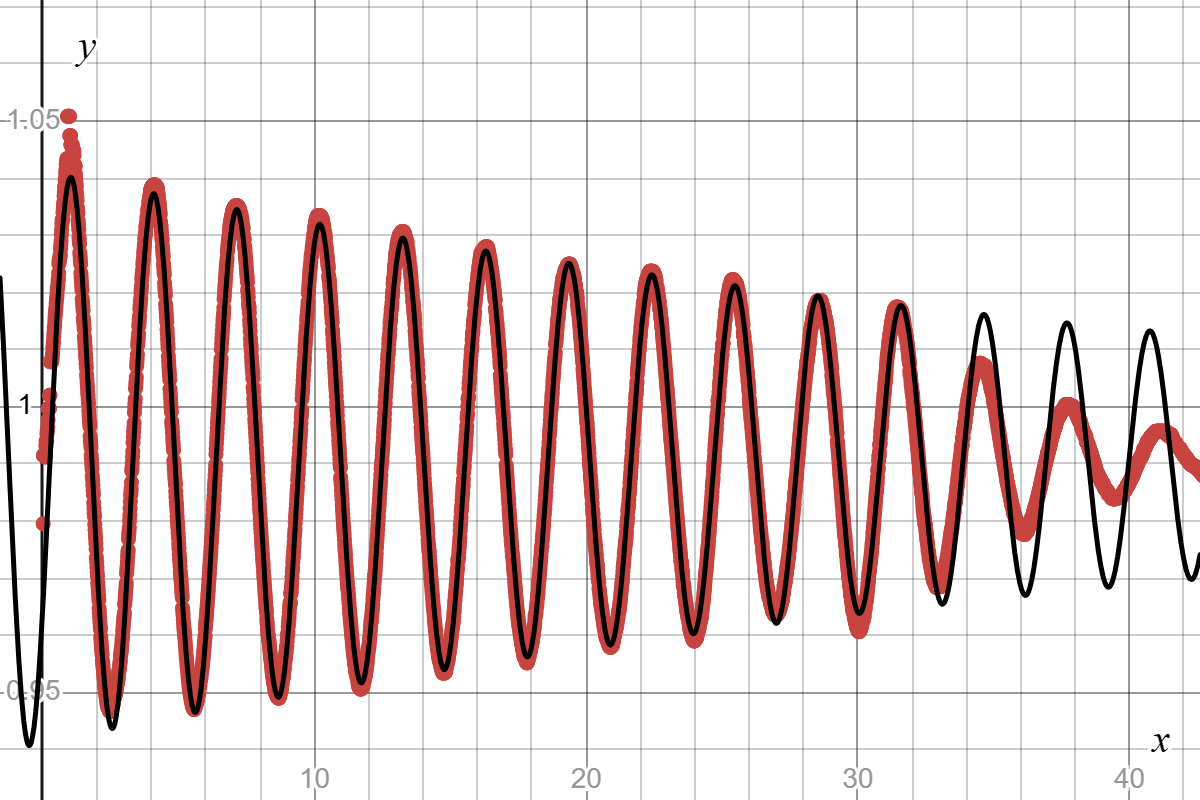
\includegraphics[width=0.7\textwidth]{images/dis_xexp_l3_t30.png}
    \caption{Зависимость уровня жидкости в момент времени $t=30$ с. от координаты с учётом затухания для длины волны $L=3$ м.}
    \label{f:dis_xexp_l3_t30}
\end{figure}

В таблице~\ref{t:fade_dis} представлены результаты анализа затухания волн.
%
Столбец кинематической вязкости $\nu$ рассчитывается по следующей формуле (приближение для $\psi \ll k$):
%
\begin{equation}
    \nu = \frac{\psi \omega}{k^2}.
\end{equation}
%
Коэффициент затухания $\psi$ рассчитывается по алгоритму выше.

\begin{table} [h!tbp]
    \centering
    \begin{threeparttable}
        \caption{Анализ затухания волн в разработанной модели для разных длин волн.}\label{t:fade_dis}
        \begin{tabular}{| p{5cm} || p{5cm} | p{5cm} |}
            \hline

            \makecell{$L$, м}  
            &  
            \makecell{Коэффициент \\ затухания $\psi$}  
            &
            \makecell{Кинематическая \\ вязкость $\nu$, $\text{м}^2/\text{с}$}

            \\
            \hline
            \hline

            \makecell{0.75} 
            &
            \makecell{0.1902}
            &
            \makecell{0.02455}

            \\
            \hline

            \makecell{1} 
            &
            \makecell{0.1727}
            &
            \makecell{0.03433}

            \\
            \hline

            \makecell{3}
            &
            \makecell{0.0200}
            &
            \makecell{0.02034}

            \\
            \hline

            \makecell{5}
            &
            \makecell{0.0132}
            &
            \makecell{0.02704}

            \\
            \hline

            \makecell{10}
            &
            \makecell{0.0059}
            &
            \makecell{0.02767}
            
            \\
            \hline
            
            \makecell{$\infty$}
            &
            \makecell{0.0039}
            &
            \makecell{-}

            \\
            \hline
        \end{tabular}
    \end{threeparttable}
\end{table}

Здесь стоит обратить внимание на снижение коэффициента затухания $\psi$ с увеличением длины волны.
%
Наименьший коэффициент затухания достигается при наибольшей длине волны --- в модели, 
где распространяется единственная волна с бесконечной длиной, солитон (генератор с уравнением~\ref{eq:nwm_solitary}).
%
Полученные значения значительно превосходят аналитическое значение кинематической вязкости ($\nu_{0} = 10^{-6}$),
что, вероятно, связано с численными диссипативными членами.

\clearpage
